\documentclass[a4paper,12pt]{report}
\addtolength{\oddsidemargin}{-1.cm}
\addtolength{\textwidth}{2cm}
\addtolength{\topmargin}{-2cm}
\addtolength{\textheight}{3.5cm}
\newcommand{\HRule}{\rule{\linewidth}{0.5mm}}
\makeindex

\usepackage{longtable}
\usepackage[pdftex]{graphicx}
\usepackage{makeidx}
\usepackage{hyperref}
\usepackage{verbatim}
\hypersetup{
    colorlinks=true,
    linkcolor=black,
    filecolor=magenta,      
    urlcolor=cyan,
}


% define the title
\author{Team Bravo}
\title{Assignment 1 Software Requirements Specification and Technology Neutral Process Design}
\begin{document}
\setlength{\parskip}{6pt}

% generates the title
\begin{titlepage}

\begin{center}
% Upper part of the page       

\includegraphics[width=1\textwidth]{../Images/University_of_Pretoria_Logo.PNG}\\[0.5cm]    
\textsc{\LARGE Department of Computer Science}\\[0.5cm]
\textsc{\Large COS 301}\\[0.5cm]
\textsc{\Large Mini Project Assignment 1}\\[0.75cm]
% Title
\HRule \\[0.4cm]
{ \huge \bfseries Software Requirements Specification \\ [0.1cm] 
	and \\ [0.5cm] Technology Neutral Process Design}\\[0.5cm]
\HRule \\[1cm]

% Author and supervisor
\textsc{\Large Team Bravo}\\[1cm]


\begin{minipage}{0.4\textwidth}
\begin{flushleft} \large
\emph{Student:}\\[0.75cm]
Daniel {King}
\end{flushleft}
\end{minipage}
\begin{minipage}{0.4\textwidth}
\begin{flushright} \large
\emph{Student number:} \\[0.75cm]
u13307607
\end{flushright}
\end{minipage}


\begin{minipage}{0.4\textwidth}
\begin{flushleft} \large
\emph{} \\
Azhar {Mohungoo }
\end{flushleft}
\end{minipage}
\begin{minipage}{0.4\textwidth}
\begin{flushright} \large
\emph{} \\
u12239799
\end{flushright}
\end{minipage}


\begin{minipage}{0.4\textwidth}
\begin{flushleft} \large
Andreas {du Preez}
\end{flushleft}
\end{minipage}
\begin{minipage}{0.4\textwidth}
\begin{flushright} \large
\emph{} \\
u12207871 
\end{flushright}
\end{minipage}

\begin{minipage}{0.4\textwidth}
\begin{flushleft} \large
Banele {Nxumalo}
\end{flushleft}
\end{minipage}
\begin{minipage}{0.4\textwidth}
\begin{flushright} \large
\emph{} \\
u12201911 
\end{flushright}
\end{minipage}


\begin{minipage}{0.4\textwidth}
\begin{flushleft} \large
Frederic {Ehlers}
\end{flushleft}
\end{minipage}
\begin{minipage}{0.4\textwidth}
\begin{flushright} \large
\emph{} \\
u11061112  
\end{flushright}
\end{minipage}


\begin{minipage}{0.4\textwidth}
\begin{flushleft} \large
Diana {Obo}
\end{flushleft}
\end{minipage}
\begin{minipage}{0.4\textwidth}
\begin{flushright} \large
\emph{} \\
u13134885
\end{flushright}
\end{minipage}


\begin{minipage}{0.4\textwidth}
\begin{flushleft} \large
Bilal {Muhammad}
\end{flushleft}
\end{minipage}
\begin{minipage}{0.4\textwidth}
\begin{flushright} \large
\emph{} \\
u13080335
\end{flushright}
\end{minipage}
\vfill

\end{center}
\end{titlepage}

\renewcommand{\thesection}{\arabic{section}}
\newpage

\tableofcontents 

\begin{center} 
\textsc{} \\[3cm]
\textsc{\Large Bravo github repository link}\\[0.5cm]
For further references, please click on this \href{https://github.com/ish1993/Bravo}{link}.
\end{center}

\newpage

\section{Introduction}

This document aims to specify the functional and non-functional requirements of a document archiving system, as specified by Ms Vreda Pieterse of the Computer Science Department.

It will serve as a means of communication between the client and developers as well as providing an elaboration and a clear discription of it's implementation specifications.

\section{Vision}

We intend to create a system that will allow authors and their co-authors to work on their research papers in an environment that reassures collaborative work, which in turn diminishes the time spent on papers with multiple authors. The following are what we plan to achieve: 

\begin{itemize}
	\item Keep track of research papers.
	\item View meta-data of research papers. 
	\item Allow multiple authors to collaborate on the same research paper. 
	\item Different levels of authority, i.e. Admin, (Co)Author, User.
	\item View and edit the details, of a text based profile, of different researchers. 
	\item Implemention as a website and an android application.
\end{itemize} 

\section{Background}

We live in a world where time is valuable. We would like to do as much as we possibly can in the shortest amount of time. And if that's not possible, we work in teams to ensure that we achieve that goal. 

Reseacher papers tend to be fairly lengthy, and if completed by only one author, it could be quite a tedious process. Hence we propose a system which would make the storage and collaboration of research articles and papers effortless by producing an archive system.

\newpage

\section{Architecture Requirements}

\subsection{Access channel requirements}
The different access channels for the system will be as follows:
\subsubsection{Web Application}
The system can be used via a web application that uses RESTful web services and bootstrap technology. The system will be fully supported on the following web browsers:
\begin{itemize}
	\item Chrome 7.0.517 and up
	\item Firefox 3.6 and up
	\item Safari 4 and up
	\item Edge
\end{itemize}
Bootstrap will be used so that the web application will also be accessible by mobile web browsers that support HTML5 and JavaScript technology.
\subsubsection{Mobile Application}
The system will also be accessible via a mobile application and will be operational on the following mobile operating systems:
\begin{itemize}
	\item Android 4.0 (Ice Cream Sandwich) and up.
\end{itemize}
\subsection{Quality requirements}
\begin{itemize}
	\item Security - The system shall identify all of its client applications before allowing them access to those enities. Possible measurement methods: Success rate in authentication, percentage of successful attacks, encryption level and probability/time/resources needed to attack the system.
	\item Usability - The degree of ease of use and training needed for end users. Possible measurement methods: Time it took a user to find a report (search functionality), percentage of deadlines met (notification functionality) and time it took a user to perform certain tasks.
	\item Auditability - The degree to which transactions can be traced. Possible measurement methods: The number and precision of logs generated in a period of time (metadata accessed/deleted/added).
	\item Portability - Measure ability of the system to run under different computing environments. Possible measurement methods: Number of targeted software environments (ie different browsers and operating systems) and proportion of platform specific functionality.
	\item Maintainability - Measures ability to make changes quickly and cost effectively. Possible measurement methods: Degree of complexity to make changes to the format of the metadata and mean time to add or change certain functionalities (ie new report types and new types of users).
	\item Availability - Percentage of time that the system is up and running correctly. Possible measurement methods: Length of time between failures and length of time needed to resume operation after a failure.
	\item Performance - Possible measurement methods: How well the system perform under high workload and number of events processed/denied in some interval of time.
\end{itemize}
\subsection{Integration requirements}

\subsection{Architecture constraints}
\begin{itemize}
	\item The platform must exist in 2 mediums, namely web and android application.
	\item It is an internal network to be used by the Computer Science department, so it need not to source any information from the web.
	\item Any form of database can be used, but the team has decided that MySQL would be the best option from the current skillset.
	\item PHP and JavaScript will be used for the web and Android Studio for the android application.
	\item The system should cater for and including 100 users as a maximum.
	\item There should be a log that records all activity on the system
\end{itemize} 

\newpage

\section{Functional requirements and application design}

\subsection{Use case prioritization}
This section specifies the level of importance of different use cases, prioritized in terms of the following 3 catogories: Critical, Important and Nice-To-Have. Each of which has a lesser importance than the previous one.

\subsubsection{Citical:}
	\begin{itemize}
		\item Server connection
		\item Database connection
		\item User gateaway
		\item Research paper management
		\item User account management
		\item Log services
	\end{itemize}
	
\subsubsection{Important:}	
	\begin{itemize}
		\item Notification Services
		\item Search Services
		\item Archival Services
	\end{itemize} 
	
\subsubsection{Nice-To-Have:}
	\begin{itemize}
		\item ???
	\end{itemize}

\subsection{Use case/Services contracts}

\subsection{Required functionality}

\subsection{Process specifications}

\subsection{Domain Model}
\begin{center}
	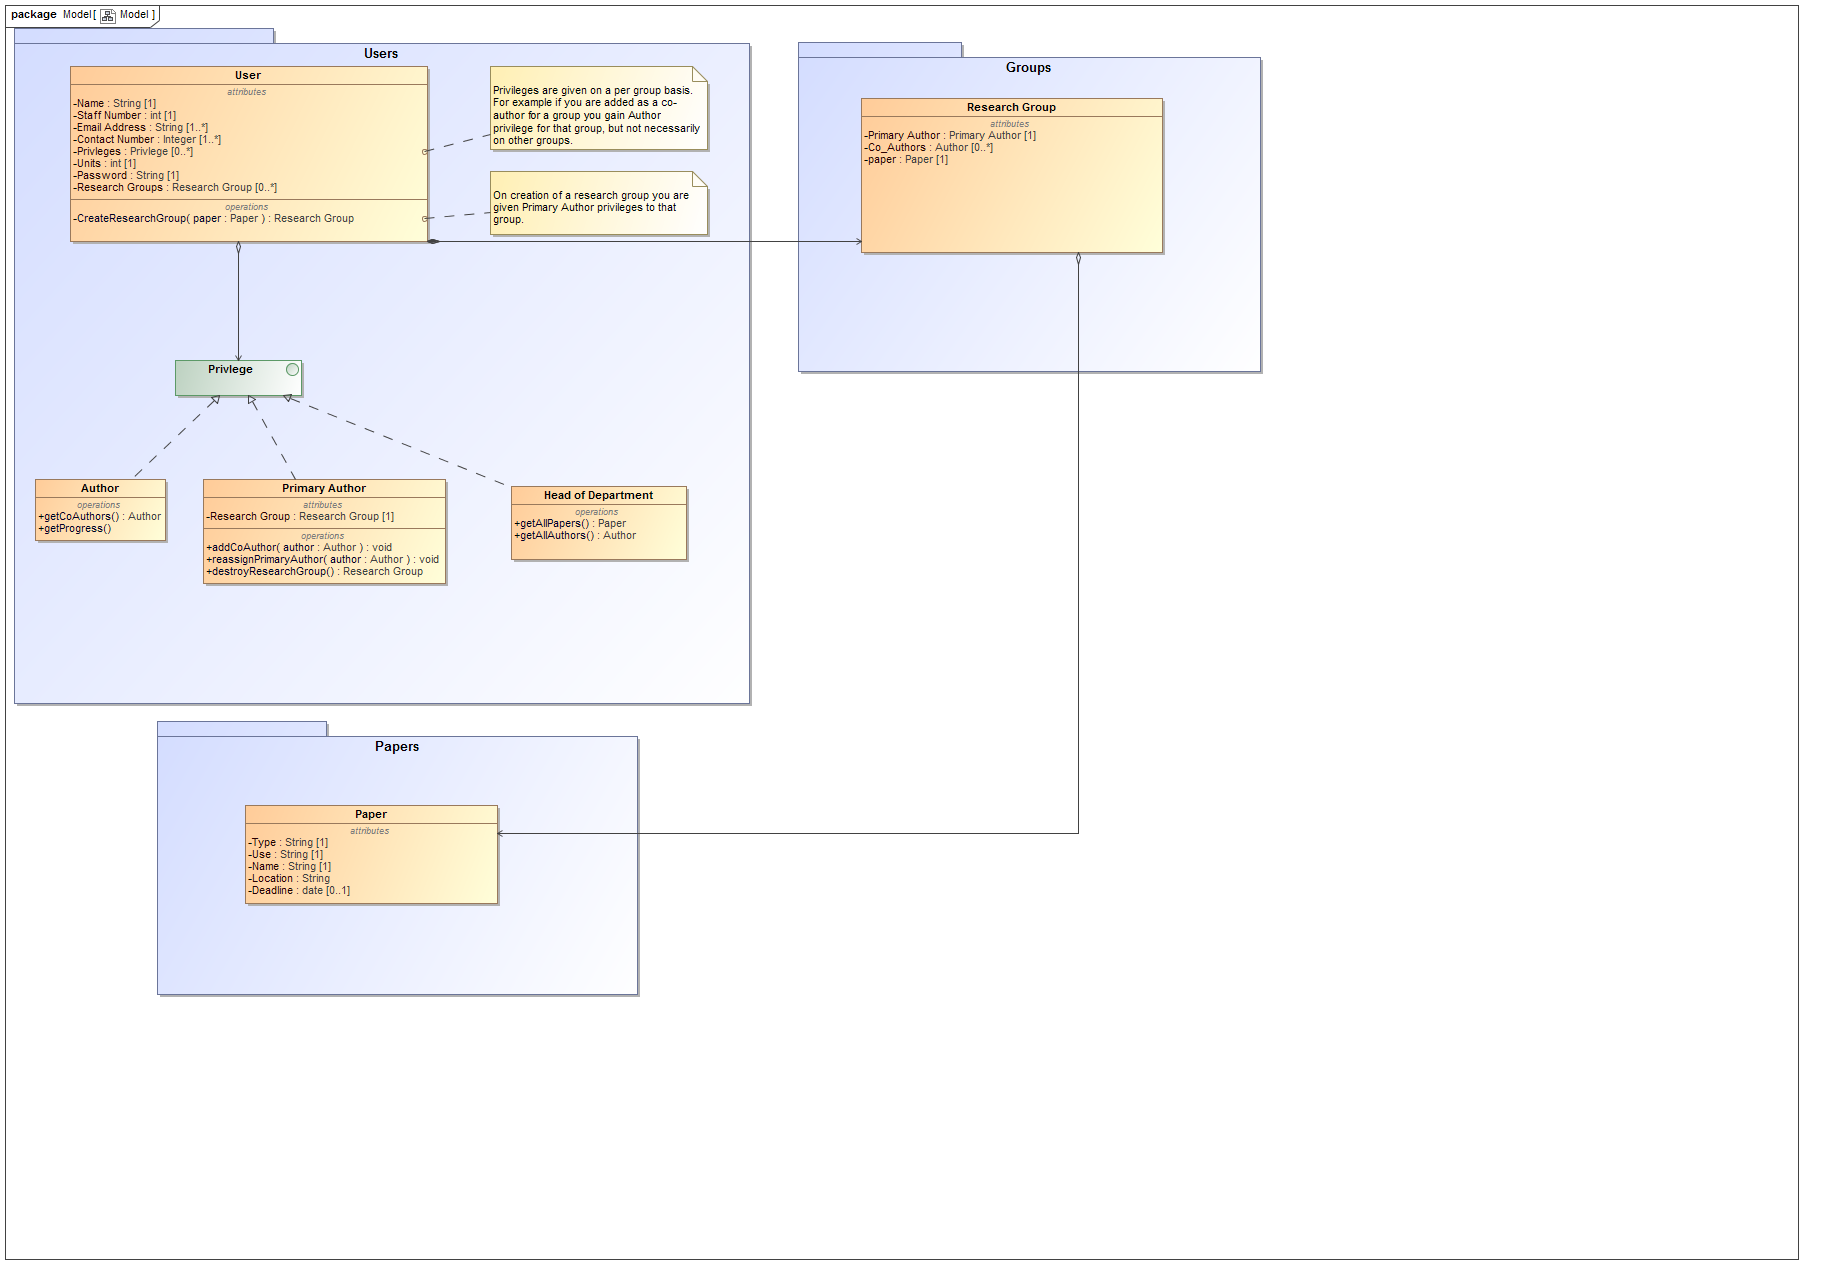
\includegraphics[width=\textwidth]{../Images/DomainModel.png}\\[0.5cm]
\end{center}



\section{Open Issues}

\newpage

\section{References}
PIETERSE, V. 2016. COS301: Mini project. In: Lecture notes issued online.  University of Pretoria. Pretoria, South Africa

\end{document}
